\chapter{Assignment 2}\label{ass2}

\section{Task 1}\label{ass2_t1}

\subsection{a}\label{ass2_t1_a}

\begin{equation}
  \begin{pmatrix}
    x_{1} \\
    y_{1}
  \end{pmatrix}
  =
  \begin{pmatrix}
    cos(\Theta_{1})  &  sin(\Theta_{1}) \\
    -sin(\Theta_{1}  &  cos(\Theta_{1}
  \end{pmatrix}
  \cdot
  \begin{pmatrix}
    L_{1} \\
    0
  \end{pmatrix}
  =
  \begin{pmatrix}
    L_{1}\cdot cos(\Theta_{1})   & 0 \\
    -L_{1}\cdot sin(\Theta_{1})  & 0
  \end{pmatrix}
  =
  \begin{pmatrix}
    L_{1}\cdot cos(\Theta_{1}) \\
    -L_{1}\cdot sin(\Theta_{1})
  \end{pmatrix}
\end{equation}

With $(x_{1}, y_{1})$ calculated in correlation to $(x, y)$, we assume $(x_{1}, y_{1})$ as the new start to calculate $(x_{2}, y_{2})$.

\begin{equation}
  \begin{pmatrix}
    x_{2} \\
    y_{2}
  \end{pmatrix}
  =
  \begin{pmatrix}
    cos(\Theta_{2})  &  -sin(\Theta_{2}) \\
    sin(\Theta_{2}  &  cos(\Theta_{2}
  \end{pmatrix}
  \cdot
  \begin{pmatrix}
    L_{2} \\
    0
  \end{pmatrix}
  =
  \begin{pmatrix}
    L_{2}\cdot cos(\Theta_{2})   & 0 \\
    L_{2}\cdot sin(\Theta_{2})  & 0
  \end{pmatrix}
  =
  \begin{pmatrix}
    L_{2}\cdot cos(\Theta_{2}) \\
    L_{2}\cdot sin(\Theta_{2})
  \end{pmatrix}
\end{equation}

\subsection{b}\label{ass2_t1_b}

The four euqations are: $x_{1} = L_{1}\cdot cos(\Theta_{1})$, $y_{1} = L_{1}\cdot sin(\Theta_{1})$, $x_{2} = L_{2}\cdot cos(\Theta_{2})$ and $y_{2} = L_{2}\cdot sin(\Theta_{2})$.
\begin{equation}
  \frac{x_{1}}{d\Theta_{1}} = -L_{1}\cdot sin(\Theta_{1})
\end{equation}
\begin{equation}
  \frac{x_{1}}{d\Theta_{2}} = 0
\end{equation}
\begin{equation}
  \frac{y_{1}}{d\Theta_{1}} = -L_{1}\cdot cos(\Theta_{1})
\end{equation}
\begin{equation}
  \frac{y_{1}}{d\Theta_{2}} = 0
\end{equation}
\begin{equation}
  \frac{x_{2}}{d\Theta_{1}} = 0
\end{equation}
\begin{equation}
  \frac{x_{2}}{d\Theta_{2}} = -L_{2}\cdot sin(\Theta_{2})
\end{equation}
\begin{equation}
  \frac{y_{2}}{d\Theta_{1}} = 0
\end{equation}
\begin{equation}
  \frac{y_{2}}{d\Theta_{2}} = L_{2}\cdot cos(\Theta_{2})
\end{equation}


\section{Task 2}\label{ass2_t2}

\subsection{a}\label{ass2_t2_a}



\subsection{b+c}\label{ass2_t2_b_c}

The coordinates have been marked in the following picture by a red eclipse.

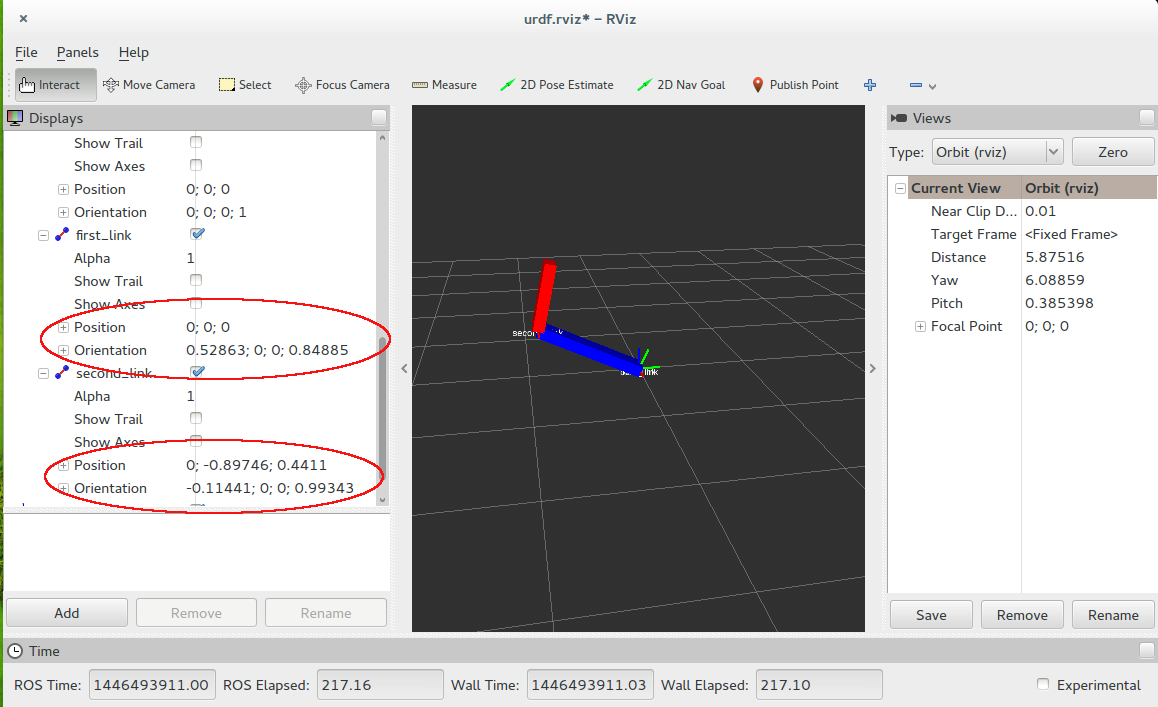
\includegraphics[width=\textwidth]{img/screen_ue2_t2_c.png}

